\documentclass{cernatsnote}
\usepackage[colorinlistoftodos]{todonotes}
\usepackage{placeins}

\title{HSE Notes}
\author{
	Author Name \; \\		
	HSE, MAGoLEGO "Social Network Analysis", SNA, Russia, Moscow
}
\email{student@hse.edu.ru}
\date{\today}

\begin{document}
\maketitle

\begin{abstract}
This document shows how to prepare for MAGoLEGO "Social Network Analysis" final exam. There are few sections in the exam and might be approximately 10-12 questions with different points assign. Time for exam - 120 minutes. Russian answers are allowed, but not advised. You are allowed to bring and use simple calculator. Computers, mobiles and materials are forbidden. Cheating or breaking exam policy leads to grade ‘0’ for the exam.
\end{abstract}
\\ \\ \\ 
\begingroup
\color{black}
\tableofcontents
\endgroup

% \pagebreak
%%%%%%%%%%%%%%%%%%%%%%%%%%%%%%%%%%%%%%%%%%%%%%%%%%%%%%%%%%%%%%%%%%%%%%%%%%%%%%%%%%%%%%%%%%%%%%%%%%%%%%%%%%%
\section{Task 1}
Construct the adjacency matrix for the following direct network:

\textbf{Solution:}
\par An adjacency matrix is defined as follows: 
\par \href{http://ceadserv1.nku.edu/longa//classes/mat385_resources/docs/matrix.html}{Let G be a graph with "n" vertices that are assumed to be ordered from v1 to vn. The n x n matrix A, in which ( the existence of an edge between two vertices vi and vj is shown by an entry of 1 in the ith row and jth column of the adjacency matrix. This entry represents a path of length 1 from vi to vj.)}
\par aij= 1 if there exists a path from vi to vj 
\par aij = 0 otherwise.

\begin{figure}[h]
\centering
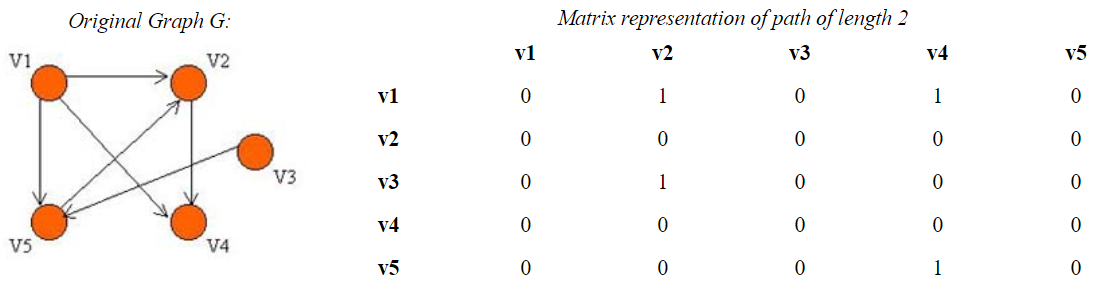
\includegraphics[width=0.8\textwidth]{images/task1.png}
\caption{\label{fig:task1} Task 1}
\end{figure}
% http://ceadserv1.nku.edu/longa//classes/mat385_resources/docs/matrix.html

%%%%%%%%%%%%%%%%%%%%%%%%%%%%%%%%%%%%%%%%%%%%%%%%%%%%%%%%%%%%%%%%%%%%%%%%%%%%%%%%%%%%%%%%%%%%%%%%%%%%%%%%%%%
\section{Task 2}
Suppose you are studying the spread of a rare disease among the set of people pictured in \href{https://www.cs.cornell.edu/home/kleinber/networks-book/networks-book-ch21.pdf}{Figure 21.22} \ref{fig:task2}. The contacts among these people are as depicted in the network in the figure, with a time interval on each edge showing when the period of contact occurred. We assume that the period of observation runs from time 0 to time 20. (This task is similar to the task in the book 21.9 \cite{task2})

\begin{figure}[ht]
\centering
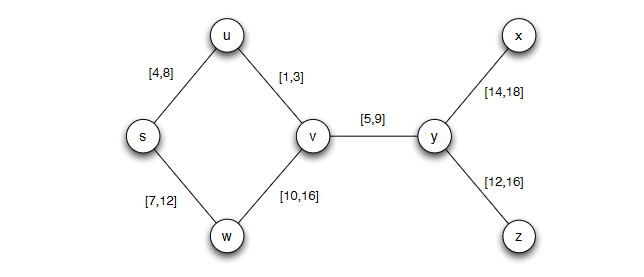
\includegraphics[width=0.8\textwidth]{images/task2.png}
\caption{\label{fig:task2} Task 2}
\end{figure}

\subsection{Task 2.1} 
if node S is the only source of decease at time 0, which nodes could potentially acquire the decease by the end of observation time? 

\textbf{Solution:} S, U W, V

\subsection{Task 2.2} 
if it is known, that everyone got infected, but there were no external sources of infection except node S, could you correct a single number (start or end of an interval) so it is possible for infection to spread over all network? 

\textbf{Solution:} 15

%%%%%%%%%%%%%%%%%%%%%%%%%%%%%%%%%%%%%%%%%%%%%%%%%%%%%%%%%%%%%%%%%%%%%%%%%%%%%%%%%%%%%%%%%%%%%%%%%%%%%%%%%%%
\section{Task 3} 
Consider an undirected network of size N in which every node has a degree k = 1. Draw possible network. How many connected components does it have? What condition should N satisfy? Write labels of nodes that will adopt behaviour A.

\textbf{Solution:} N/2 == 0 (even), connected components  (1)----(2)   (3)------(4)
%%%%%%%%%%%%%%%%%%%%%%%%%%%%%%%%%%%%%%%%%%%%%%%%%%%%%%%%%%%%%%%%%%%%%%%%%%%%%%%%%%%%%%%%%%%%%%%%%%%%%%%%%%%
\section{Task 4} 
Consider the model from Chapter 19 in Figure 19.29 \cite{task4} for the diffusion of a new behavior through a social network. Recall the model of influence propagation. All nodes follow behaviour B and have threshold q = 2/5. At some point nodes C and D have switched to behaviour A. Write labels of nodes that will adopt behaviour A.

\begin{figure}[h]
\centering
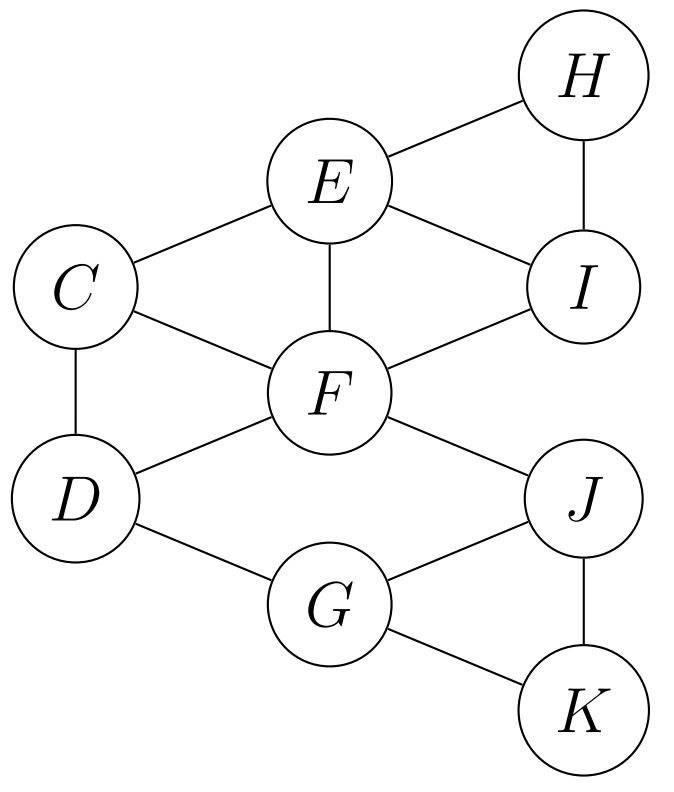
\includegraphics[width=0.4\textwidth]{images/task4.png}
\caption{\label{fig:task4} Task 4}
\end{figure}

\textbf{Solution:} C, D, E, F, H, I
%%%%%%%%%%%%%%%%%%%%%%%%%%%%%%%%%%%%%%%%%%%%%%%%%%%%%%%%%%%%%%%%%%%%%%%%%%%%%%%%%%%%%%%%%%%%%%%%%%%%%%%%%%%
\section{Task 5} 
For the given network find

\begin{figure}[h]
\centering
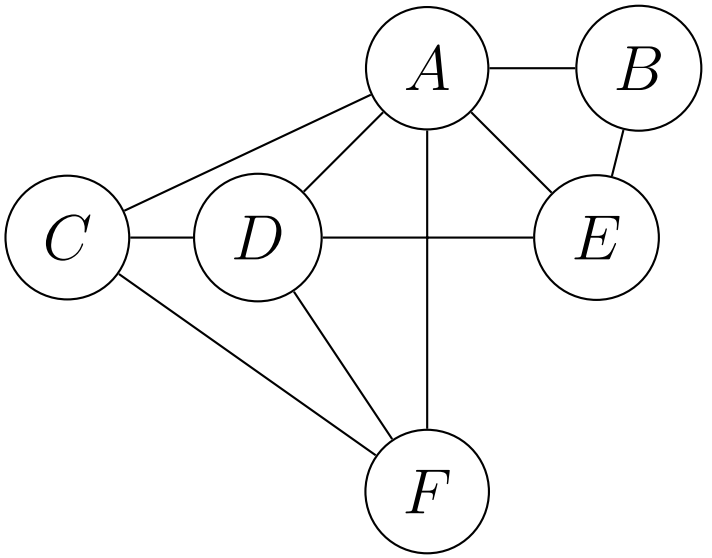
\includegraphics[width=0.4\textwidth]{images/task5.png}
\caption{\label{fig:task5} Task 5}
\end{figure}

\subsection{Task 5.1} 
Network diameter
\textbf{Solution:} 2

\subsection{Task 5.2} 
Max degree
\textbf{Solution:} 4

\subsection{Task 5.3} 
Min degree
\textbf{Solution:} 2

\subsection{Task 5.4} 
The node with the smallest clustering coefficient
\textbf{Solution:} B

\subsection{Task 5.5} 
The node with the largest clustering coefficient
\textbf{Solution:} A, C, E
%%%%%%%%%%%%%%%%%%%%%%%%%%%%%%%%%%%%%%%%%%%%%%%%%%%%%%%%%%%%%%%%%%%%%%%%%%%%%%%%%%%%%%%%%%%%%%%%%%%%%%%%%%%
\section{Task 6} 
Given the following graph Plot degree distribution (histogram) and answer the question whether it satisfies Power-Law

\begin{figure}[h]
\centering
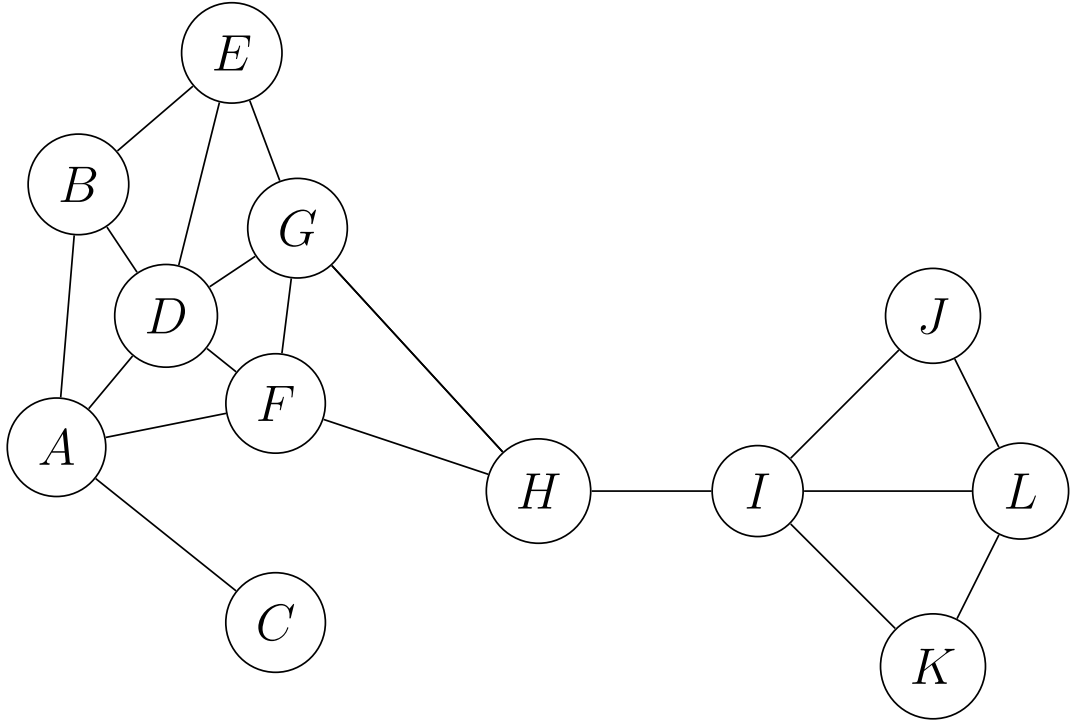
\includegraphics[width=0.6\textwidth]{images/task6.png}
\caption{\label{fig:task6} Task 6}
\end{figure}

\textbf{Solution:}  Make a diagram - node degree (horizontal) and number of nodes (vertical) - as a result, you will get a distribution, which would not satisfy Power Law  \href{http://networksciencebook.com/chapter/4#ultra-small}{Task 6 - Solution}

\begin{figure}[h]
\centering
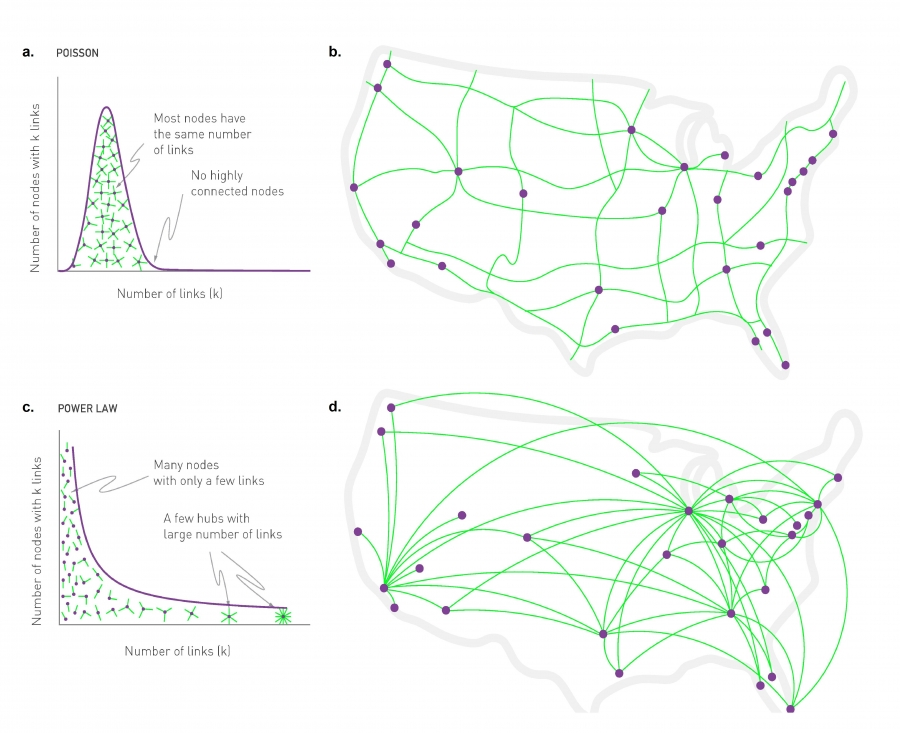
\includegraphics[width=0.8\textwidth]{images/figure-4-6.jpg}
\caption{\label{fig:figure-4-6.jpg} Task 6 - Solution}
\end{figure}

\begin{table}[h!]
\begin{tabular}{|l|l|l|l|l|l|l|l|l|l|l|l|l|}
\hline
Name of node & A & B & C & D & E & F & G & H & I & J & K & L \\ \hline
Degree       & 4 & 3 & 1 & 5 & 3 & 4 & 4 & 3 & 4 & 2 & 2 & 3 \\ \hline
\end{tabular}
\end{table}

% http://networksciencebook.com/chapter/4#ultra-small
%%%%%%%%%%%%%%%%%%%%%%%%%%%%%%%%%%%%%%%%%%%%%%%%%%%%%%%%%%%%%%%%%%%%%%%%%%%%%%%%%%%%%%%%%%%%%%%%%%%%%%%%%%%
\section{Task 7} 
Find a 3-core of the given network
\begin{figure}[h!]
\centering
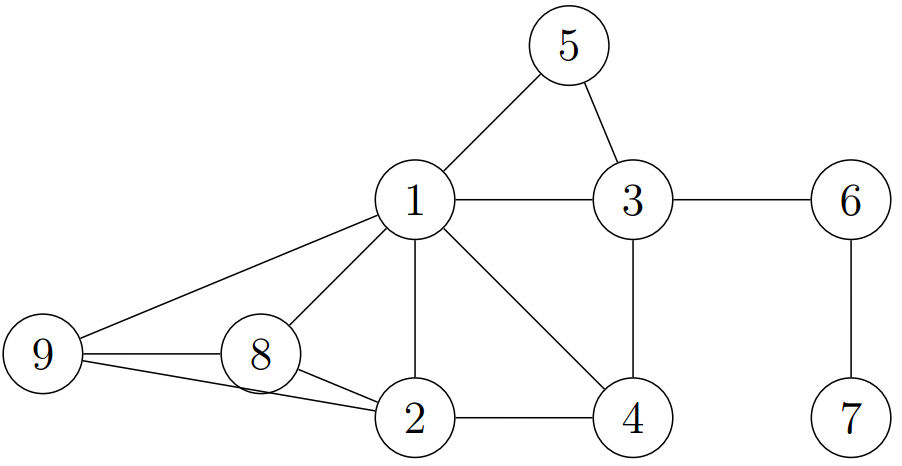
\includegraphics[width=0.6\textwidth]{images/task7.png}
\caption{\label{fig:task7} Task 7}
\end{figure}

\textbf{Solution:}  (1, 2, 8, 9)
%%%%%%%%%%%%%%%%%%%%%%%%%%%%%%%%%%%%%%%%%%%%%%%%%%%%%%%%%%%%%%%%%%%%%%%%%%%%%%%%%%%%%%%%%%%%%%%%%%%%%%%%%%%
\section{Task 8} 
Compute Hubs and Authorities values (HITS) for the given directed graph G=( 
\begin{math} 
\left\{ A,B,C \right\},
\end{math}
\begin{math} 
\left\{ (C,A),(C,B),(A,B),(B,A) \right\}).
\end{math}
Normalize the results using Euclidean norm.

\begin{figure}[h!]
\centering
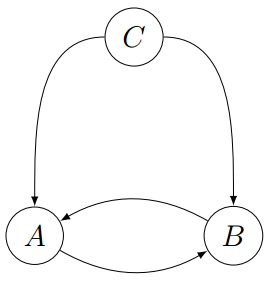
\includegraphics[width=0.3\textwidth]{images/task8.png}
\caption{\label{fig:task8} Task 8}
\end{figure}

%%%%%%%%%%%%%%%%%%%%%%%%%%%%%%%%%%%%%%%%%%%%%%%%%%%%%%%%%%%%%%%%%%%%%%%%%%%%%%%%%%%%%%%%%%%%%%%%%%%%%%%%%%%
\section{Task 9} 
For the four networks indicate assortative and disassortative cases with respect to degree and closeness centrality metrics

\begin{figure}[h!]
\centering
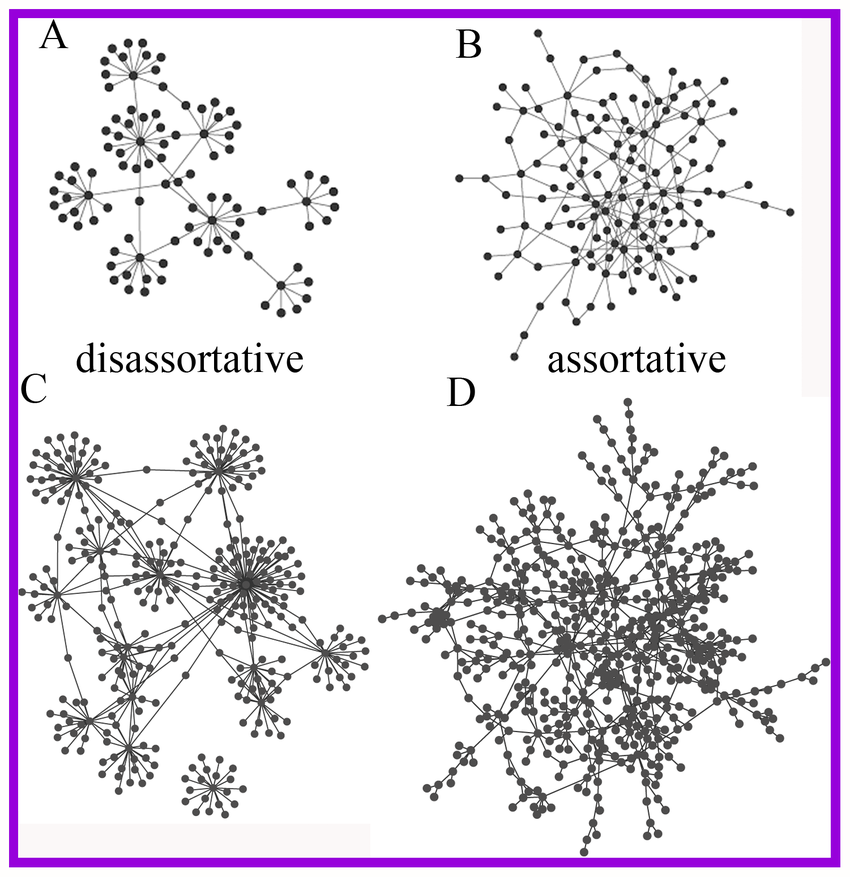
\includegraphics[width=0.8\textwidth]{images/task9.png}
\caption{\label{fig:task9} Task 9}
\end{figure}

\textbf{Solution:}  A. Disassortative network by degree - uniform (low degree adjacent to high degree) (high degree nodes connected to low degree nodes, star-like structure)

B.  Assortative network by degree - core of high degrees and a periphery of low degrees (interconnected high degree nodes - core, low degree nodes - periphery)

\href{https://doi.org/10.1371/journal.pone.0028322.g001}{Disassortative and assortative networks. Schematic illustration of a disassortative network (A) and an assortative network (B). C. The 15 best connected proteins and their direct links to other proteins of yeast protein network constructed by proteins localized in nucleus. D. The rest of network after removal of the 15 best connected nodes. Nodes disconnected to the largest component are not shown. A predominant feature of B and D is the over-abundance of links between low connected nodes.} 

%%%%%%%%%%%%%%%%%%%%%%%%%%%%%%%%%%%%%%%%%%%%%%%%%%%%%%%%%%%%%%%%%%%%%%%%%%%%%%%%%%%%%%%%%%%%%%%%%%%%%%%%%%%
\section{Task 10} 
Calculate the number of nodes reachable in d steps from the central node of a Cayley tree ( every node has a degree k). Example of a tree with k = 3 is shown below:

\begin{figure}[h!]
\centering
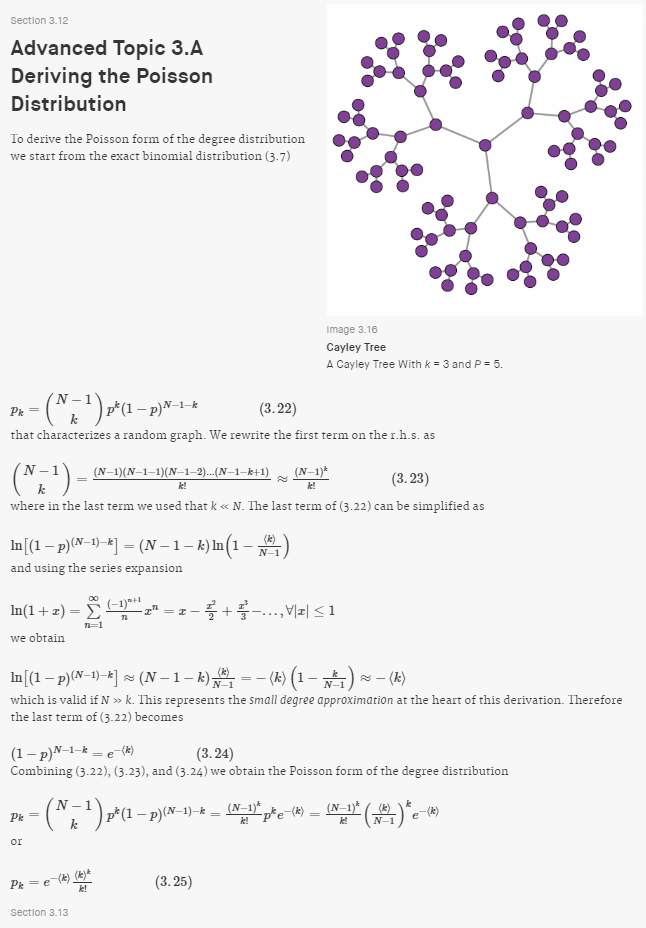
\includegraphics[width=0.8\textwidth]{images/task10.png}
\caption{\label{fig:task9} Task 10}
\end{figure}

\par \textbf{Solution:} \href{http://networksciencebook.com/chapter/3#advanced-a}{Task 10}
\par Cayley Tree
\par A Cayley tree is a symmetric tree, constructed starting from a central node of degree k. Each node at distance d from the central node has degree k, until we reach the nodes at distance P that have degree one and are called leaves (see Image 3.16 for a Cayley tree with k = 3 and P = 5.)
%%%%%%%%%%%%%%%%%%%%%%%%%%%%%%%%%%%%%%%%%%%%%%%%%%%%%%%%%%%%%%%%%%%%%%%%%%%%%%%%%%%%%%%%%%%%%%%%%%%%%%%%%%%
\section{Task 11} 
In which case (a,b,c,d) modularity will be the largest? Why? Nodes are colored according to the communities they are assigned to. Compute Modularity

\textbf{Higher Modularity Implies Better Partition} 

\par The higher is M for a partition, the better is the corresponding community structure. Indeed, in Image 9.16a the partition with the maximum modularity (M=0.41) accurately captures the two obvious communities. A partition with a lower modularity clearly deviates from these communities (Image 9.16b). Note that the modularity of a partition cannot exceed one [31,32].

\textbf{Zero and Negative Modularity}

\par By taking the whole network as a single community we obtain M=0, as in this case the two terms in the parenthesis of (9.12) are equal (Image 9.16c). If each node belongs to a separate community, we have Lc=0 and the sum (9.12) has nc negative terms, hence M is negative (Image 9.16d).

\par \textbf{Modularity} - To better understand the meaning of modularity, we show M defined in (9.12) for several partitions of a network with two obvious communities.

\par \textbf{a.	Optimal Partition} - The partition with maximal modularity M = 0.41 closely matches the two distinct communities.
\par \textbf{b.	Suboptimal Partition} - A partition with a sub-optimal but positive modularity, M = 0.22, fails to correctly identify the communities present in the network.
\par \textbf{c.	Single Community} - If we assign all nodes to the same community we obtain M=0, independent of the network structure.
\par \textbf{d.	Negative Modularity} - If we assign each node to a different community, modularity is negative, obtaining M=-0.12.
\par \textbf{We can use modularity} to decide which of the many partitions predicted by a hierarchical method offers the best community structure, selecting the one for which M is maximal. This is illustrated in Image 9.12f, which shows M for each cut of the dendrogram, finding a clear maximum when the network breaks into three communities.

% http://networksciencebook.com/chapter/9#modularity

\begin{figure}[h!]
\centering
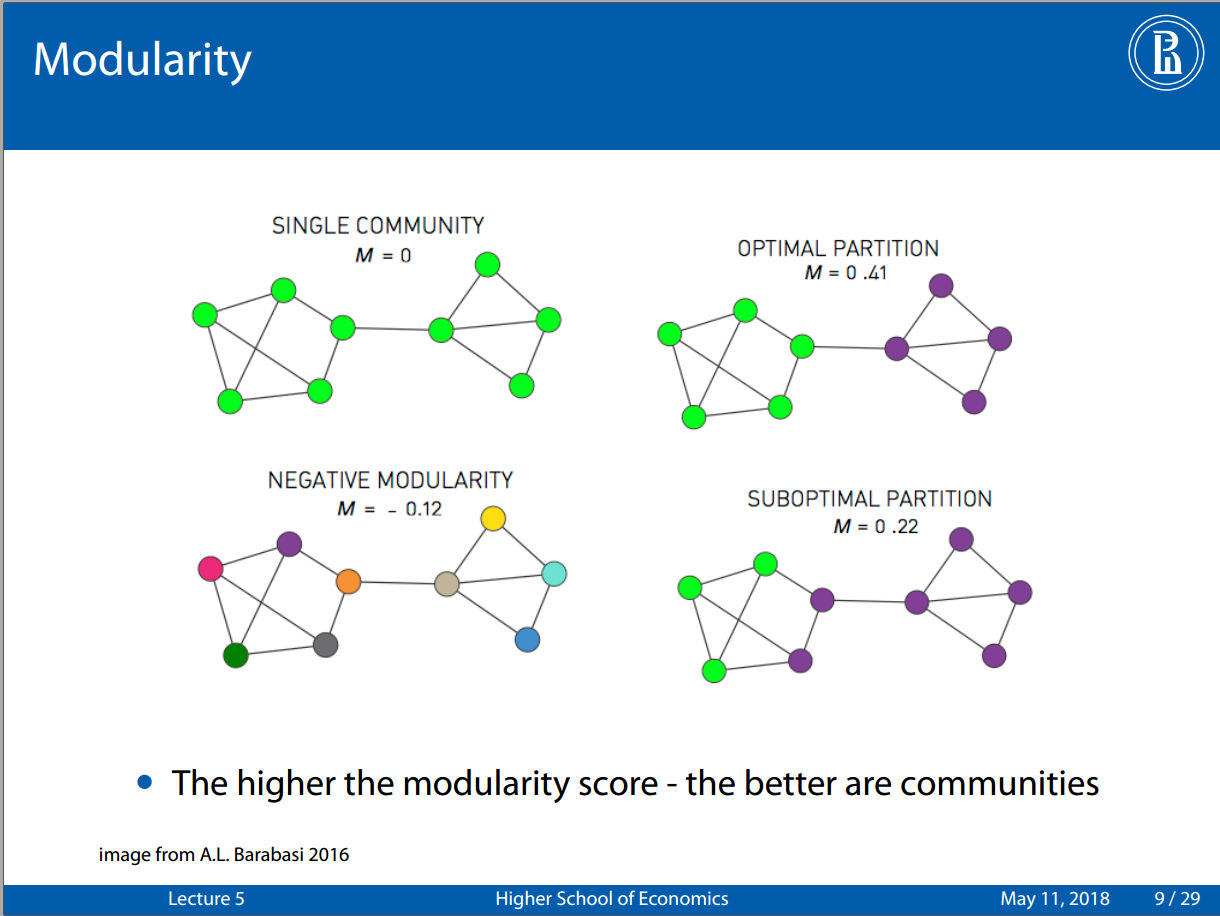
\includegraphics[width=0.8\textwidth]{images/task11.png}
\caption{\label{fig:task9} Task 11}
\end{figure}



\bibliography{references}
\bibliographystyle{plain}

\end{document}



%%%%%%%%%%%%%%%%%%%%%%%%%%%%%%%%%%%%%%%%%%%%%%%%%%%%%%%%%%%%%%%%%%%%%%%%%%%%%%%%%%%%%%%%%%%%%%
%%%%%%%%%%%%%%%%%%%%%%%%%%%%%%%%%%%%%%%%%%%%%%%%%%%%%%%%%%%%%%%%%%%%%%%%%%%%%%%%%%%%%%%%%%%%%%
%%%%%%%%%%%%%%%%%%%%%%%%%%%%%%%%%% Below is an example from CERN, Thank You for cool template!


(See ref. \cite{MADX}). The reason is that a sector magnet definition can also model a rectangular magnet, so it is easier just to use the sector bending magnet definition. The sector magnet definition is characterized by it's arc length "$L$", it's bending angle "$\phi$" and it's pole-face angles "$e1$ and $e2$", (see Figure \ref{fig:StandardMagnetLayout}). \\
\begin{figure}[ht]
\centering
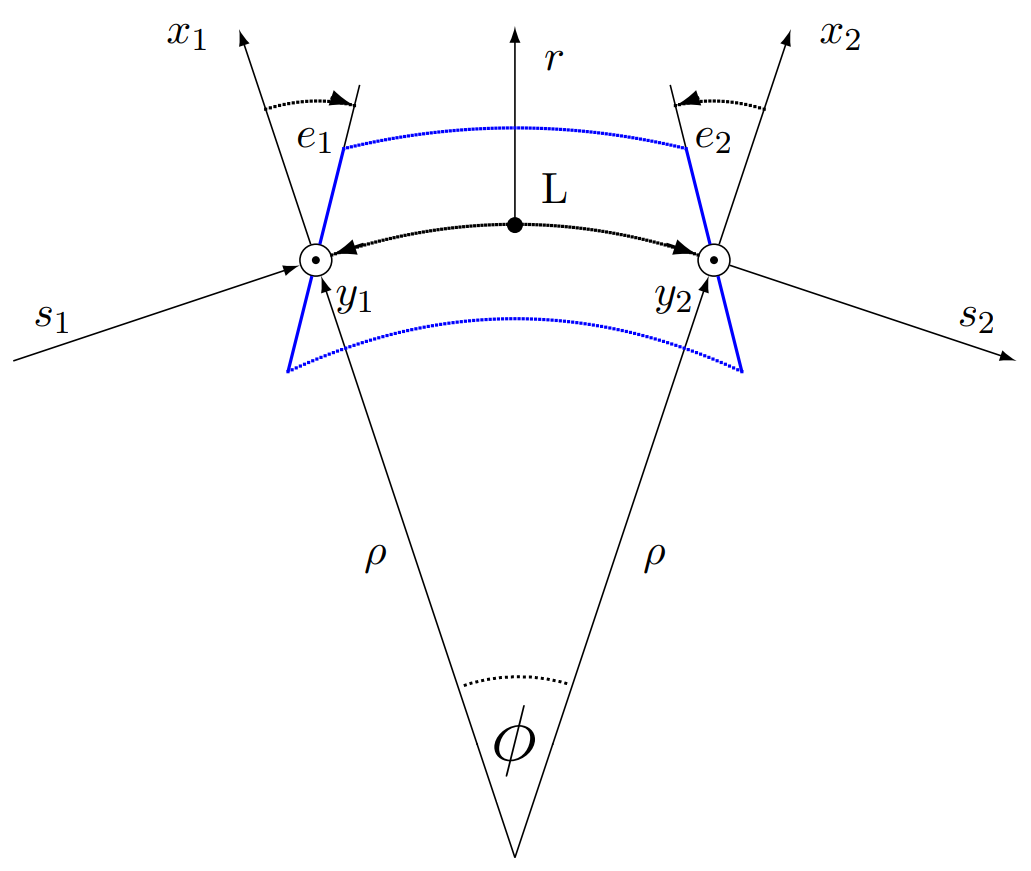
\includegraphics[width=0.8\textwidth]{images/StandardMagnetLayout.png}
\caption{\label{fig:StandardMagnetLayout} Standard magnet layout for a sector bending magnet}
\end{figure}

Looking at the definition of a sector magnet in MADX:
\begin{align*} 
label: &SBEND, L=real, ANGLE=real, TILT=real, \\
&K0=real, K1=real, K2=real, K1S=real, \\
&E1=real, E2=real,\\
&FINT=real, FINTX=real, HGAP=real, H1=real, H2=real, THICK=logical;
\end{align*}

In the above formula "L" is the arc length, "ANGLE" is the bending angle "$\phi$" and "E1" \& "E2" are the pole face angles.

\pagebreak

\noindent
\textit{NB! Please note that for Fig.\ref{fig:StandardMagnetLayout}, the definition of a positive bending angle as well as the pole face angles depends on the charge of the particle that moves through the bending magnet. If a positively charged particle is bent to the right, then the bending angle is positive. If a negatively charged particle is bent to the right, then the bending is negative.} \\ \\

The arc length $L$ is extremely important for survey calculations and is equal to the increase in the s variable from the entry to the exit of the magnet. The entry and exit points of the magnet is called ENTRE and SORTIE, which are the names defined in the survey database (See ref. \cite{GEODE})

For survey calculations, we use four different types of magnet length. These four different magnet lengths are used by other groups (see Figure \ref{fig:3Length}):

\begin{figure}[ht]
\centering
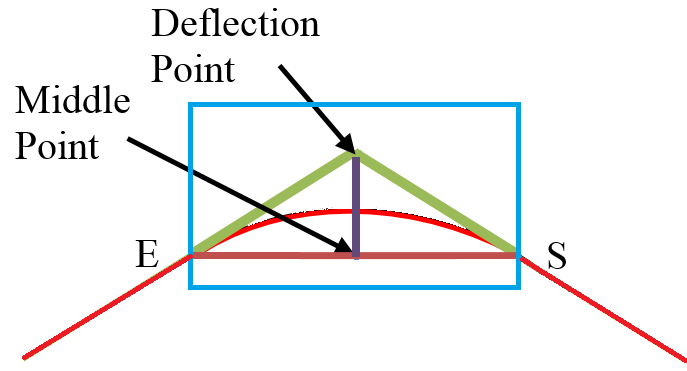
\includegraphics[width=0.9\textwidth]{images/3Length.png}
\caption{\label{fig:3Length} Definition of three different length for a bending magnet. \color{blue}The rectangular blue box is the bending magnet itself  \color{red}The Red circular line from point E to point S is the arc length. \color{brown} The straight brown line from point E to point S is the magnetic length. arc length. \color{green} The two angled green straight lines from point E to point S is the length via the deflection point.}
\end{figure}

\begin{enumerate}
\item \textbf{The physical length}. This is length given in layout drawings. It is only used for survey calculations but never for optics calculations. But, as the survey group also accepts the magnetic length as a basis for survey calculations, then in the magnetic length is always used for all types of calculation and the physical length is basically never used.
\item \textbf{The magnetic length}. This is used by the MADX program for optics calculations, but can also be accepted as a basis for survey calculations. The magnetic length, as a concept, is equivalent to the physical length. The magnetic length is calculated from magnet measurements, and the formula for the magnetic length is: $L_{Mag}=\frac {\int_{ }^{ } B dl}{B_{Max}}$, where $B_{Max}$ is the maximum B field in the center of the magnet.
\item \textbf{The arc length}. This is used by the MADX program. It is the length of the beam trajectory and is the length given in the SBEND command. It is also called the path length.
\item \textbf{The straight line length between the ENTRY and SORTIE points}. This was in the past used by the GEODE survey program. However, recently GEODE has converted to use the arc length, but there are still instances where the ENTRY/SORTIE length is still used. The survey program could in certain instances base this length on either the physical length or the magnetic length.
\end{enumerate}

\noindent \textit{NB! Please be very careful to check whether a physical length or a magnetic length is used. Check e.g. with the NORMA magnet database. See ref.\cite{NORMA} } 

\section{How to position a straight vacuum chamber to maximize aperture for the beam}
Looking at Figure \ref{fig:3Length}, we see a beam going from point E to point S, following the red circular line, and we imagine that it passes inside a straight vacuum pipe (this could be represented by the blue square rectangle). In order to maximize the aperture, then the middle of the vacuum chamber should be exactly between the maximum extended circular arc and the ES line. Seen from the center of circle with $ \rho$ as the bending radius, the middle of the vacuum chamber should then be the average between $ \rho $ and the ES line (= $ \rho *Cos(\frac {\alpha}{2} )$ ), i.e. equal to:
$ \frac{\rho}{2} * (1 - Cos[\frac{\alpha}{2}])$ above the E-S line. \\

This formula is independent of the how the layout of bending magnet is done (see the next section with the three layouts of a rectangular magnet). 

\pagebreak

\section{Three layouts for a rectangular magnet}

\subsection{The standard magnet layout}

\begin{figure}[ht]
\centering
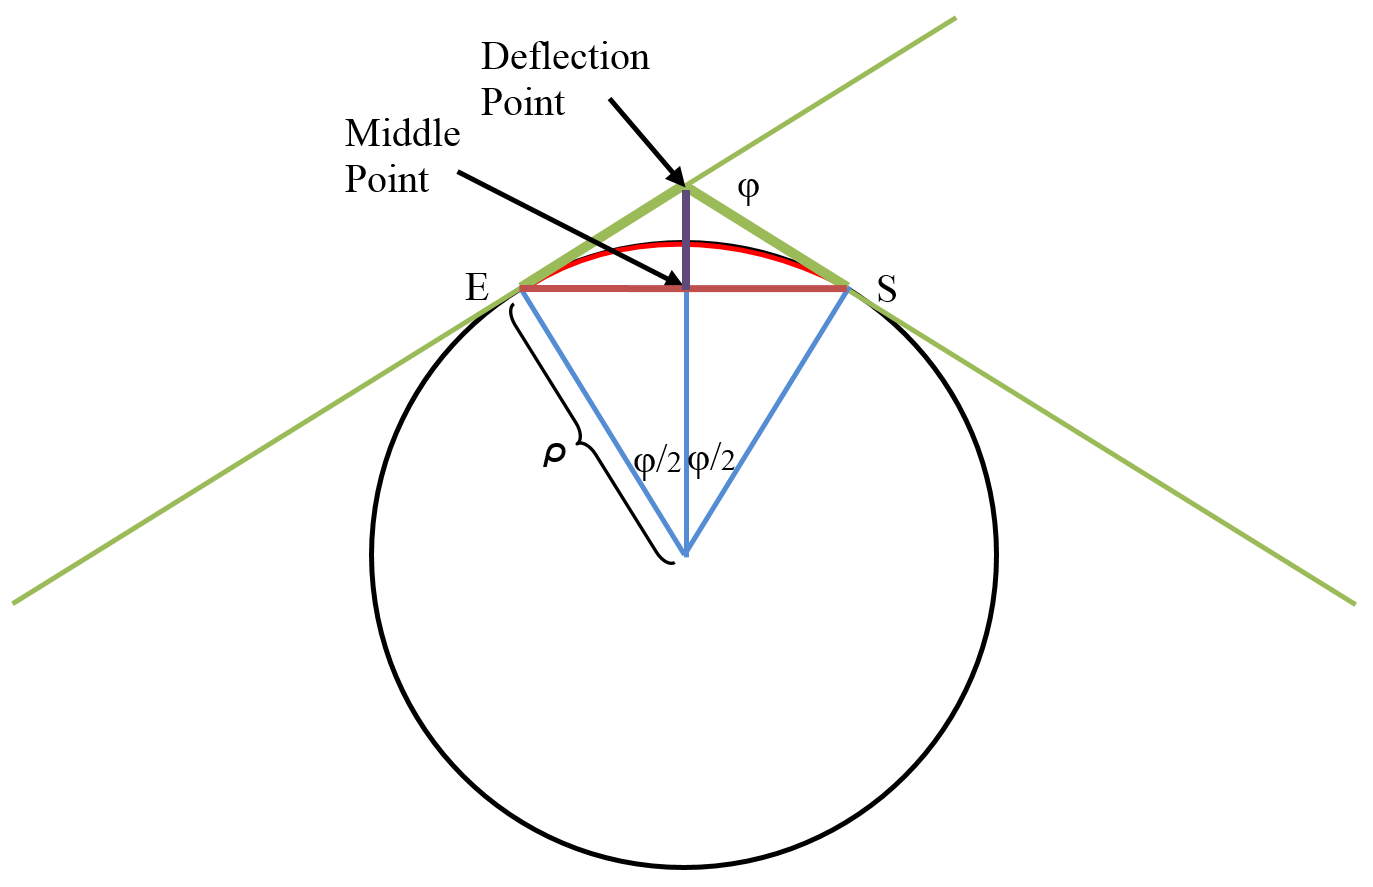
\includegraphics[width=0.9\textwidth]{images/StandarMagnet_DeflectionPoint.png}
\caption{\label{fig:StandarMagnet_DeflectionPoint} 
         Calculation of path length for standard magnet layout.}
\end{figure}

\FloatBarrier

\begin{align*} 
\begin{split}
 L_{arc} & =\rho \cdot \phi \\
 L_{Dfl} & =\frac{L}{Cos(\frac{\phi}{2})} = 2\cdot \rho \cdot Tan(\frac{\phi}{2}) = 2 \cdot L_{arc} \cdot \cfrac{Tan(\frac{\phi}{2})}{\phi} \\
  L_{ES} & =L = \rho \cdot 2 \cdot Sin(\frac{\phi}{2})  \\ \\
 where \\
 L_{arc} & = path\ length\ i.e\ the\ length\ of \ the \ beam\ trajectory \\
 L_{Dfl} & = Length\ via\ deflection\ point\ \\
 \rho & = \frac{L}{2\cdot Sin(\frac{\phi}{2})} \\
  & = bending\ radius\ of\ the\ rectangular\ bending\ magnet \\
  \phi & = bending\ angle\ of\ the\ rectangular\ bending\ magnet \\
 L & = magnetic\  length\ of\ the\ rectangular\ bending\ magnet \\
\end{split}
\end{align*}

\pagebreak

\subsection{Rectangular bending magnet with zero pole phase angle at ENTRE}

\begin{figure}[ht]
\centering
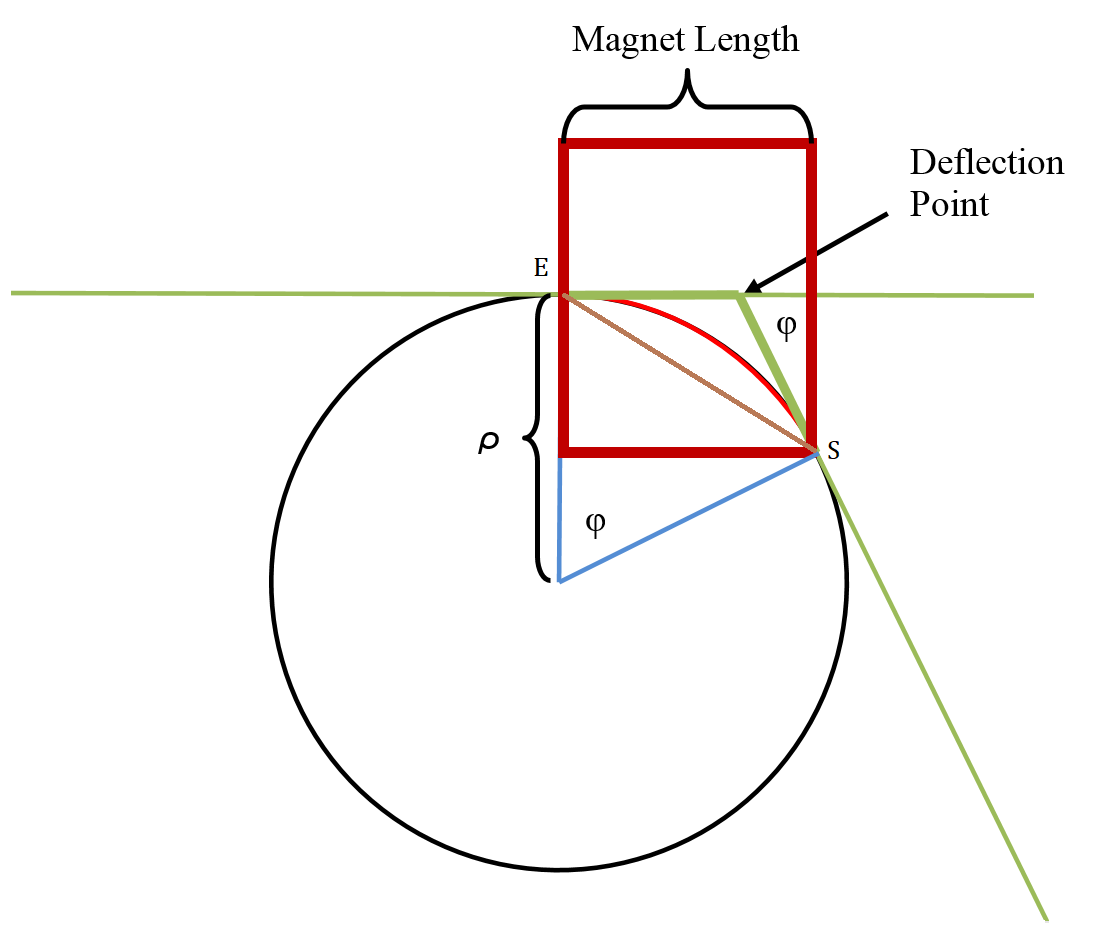
\includegraphics[width=0.7\textwidth]{images/BendingMagnet_Aligned_Entre.png}
\caption{\label{fig:BendingMagnet_Aligned_Entre} 
         Calculation of path length for magnet aligned with ENTRE.}
\end{figure}
\FloatBarrier

\begin{align*} 
\begin{split}
 L_{arc} & =\rho \cdot \phi \\
 L_{Dfl} & = 2\cdot \rho \cdot Tan(\frac{\phi}{2}) = \frac{L}{\ {Cos(\frac{\phi}{2})}^2}  \\
  L_{ES} & = \rho \cdot 2 \cdot Sin(\frac{\phi}{2})  \\ \\
 where \\
 L_{arc} & = path\ length\ i.e\ the\ length\ of \ the \ beam\ trajectory \\
 L_{Dfl} & = Length\ via\ deflection\ point\ \\
 \rho & = \frac{L}{Sin(\phi)} \\
  & = bending\ radius\ of\ the\ rectangular\ bending\ magnet \\
  \phi & = bending\ angle\ of\ the\ rectangular\ bending\ magnet \\
 L & = magnetic\  length\ of\ the\ rectangular\ bending\ magnet \\
\end{split}
\end{align*}

\pagebreak

\subsection{Rectangular bending magnet arbitrary pole phase angles}

\begin{figure}[ht]
\centering
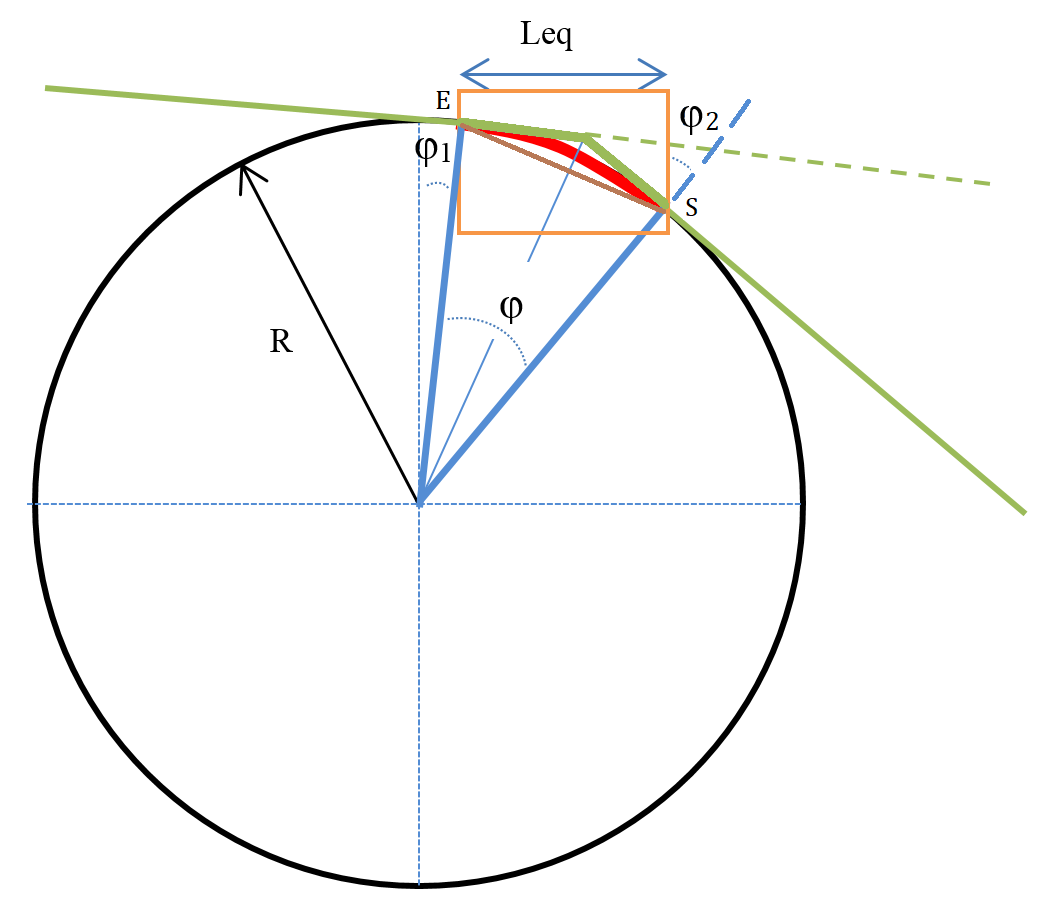
\includegraphics[width=0.7\textwidth]{images/BendingMagnet_Arbitrary_Angles.png}
\caption{\label{fig:BendingMagnet_Arbitrary_Angles} 
Calculation of path length for magnet with arbitrary polephase angles. In the above Figure \ref{fig:BendingMagnet_Arbitrary_Angles} the poleface angle at the ENTRY equal -$\phi1$ ($E1=-\phi1$), while the poleface angle at SORTIE equals $\phi2$ ($E2=\phi2$). From geometric considerations it can be seen that the sum of the poleface angles $E1+E2=\phi$  }
\end{figure}
\FloatBarrier

\begin{align*} 
\begin{split}
 L_{arc} & =\rho \cdot \phi \\
 L_{Dfl} & = 2\cdot \rho \cdot Tan(\frac{\phi}{2})   \\
  L_{ES} & = \rho \cdot 2 \cdot Sin(\frac{\phi}{2})  \\ \\
 where \\
 L_{arc} & = path\ length\ i.e\ the\ length\ of \ the \ beam\ trajectory \\
 L_{Dfl} & = Length\ via\ deflection\ point\ \\
 \rho & = \frac{L}{Sin(E1)+Sin(E2)} \\
  & = bending\ radius\ of\ the\ rectangular\ bending\ magnet \\
  \phi & = bending\ angle\ of\ the\ rectangular\ bending\ magnet \\
 L & = magnetic\  length\ of\ the\ rectangular\ bending\ magnet \\
\end{split}
\end{align*}
